\section{Practica ejercicios}
\subsection*{Enunciado ejercicio}
Una empresa de desarrollos electrónicos planea lanzar al mercado el instrumento universal de diagnóstico 
que ha bautizado con el nombre de “RobotDoc”. Para este proyecto nos ha contratado el desarrollo del 
software y nos ha pedido una primera impresión. 

\medskip
El aparato será una especie de robot ambulante y tendrá como parte de su arquitectura una computadora 
donde se ejecutará el software, una carcaza que le dará usabilidad desde el punto de vista ergonométrico y un
componente electrónico que permite conectarse con otros instrumentos que no poseen medios de 
comunicación estándard como las computadoras (RJ45, USB, etc.). Está orientado a centros de salud que no 
poseen un sistema integrado de información.

\medskip
Se pensó a “RobotDoc” como un recolector de información de los diferentes consultorios/laboratorios donde 
se realizan los siguientes estudios: electroencefalograma, electrocardiograma, resonancia magnética, rayos X
y electromiograma. En estos casos el aparato se conecta con otros instrumentos y consume datos tales como 
señales muestreadas. En el caso de los laboratorios se conecta con las computadoras y consume datos de 
informes.

\medskip
El operador se desplaza a cada lugar y al tomar los datos ingresa información del paciente de manera que al 
final del recorrido por diferentes áreas del hospital queda agrupada la información por paciente. Es decir que 
para cada paciente habrá un conjunto de estudios con los cuales los diferentes médicos que lo atiendan 
podrán elaborar un diagnóstico utilizándola. 

\medskip
“RobotDoc” es compartido por varios médicos, los cuales acceden a él y elaboran su diagnóstico con el 
enfoque de su especialidad. Para este fin “RobotDoc” debe presentar la funcionalidad de “diagnosticar” con 
enfoques preestablecidos para cada especialidad (gastroenterología, cardíaco, clínico, neurológico, etc.). Los 
diagnósticos no podrán ser realizados si no fue recolectada la información de todos los estudios solicitados. 
Aquellos estudios que daten de más de 15 días deberán repetirse, es decir que quedan invalidados para ser 
utilizados en la elaboración de un diagnóstico, solo serán usados como informativos. Cada paciente tendrá 
una historia clínica conformada por todos los estudios realizados y los diagnósticos realizados.
La información de los diferentes estudios deben poder relacionarse a partir de un conjunto determinado de 
algoritmos que aún no fueron entregados. Esta funcionalidad es una especie de asistencia al médico que 
permiten detectar diferentes fenómenos, medir distintas magnitudes, correlacionar sucesos de diferentes 
estudios, procesar señales e imágenes. 

\medskip
Los diagnósticos incluirán posibles causas, explicaciones, recomendaciones y prescripciones realizadas por 
el médico especialista en base a la información recolectada y procesada. Los profesionales para utilizarlos 
deben registrarse previamente y serán agrupados por el administrador según su especialidad. Las secretarias 
de las áreas del hospital podrán acceder a los estudios e imprimirlos para ser entregados a los pacientes. 
Todos los usuarios deben estar agrupados a efectos de poder acceder al uso.

\medskip
Se cree que la experiencia compartida por profesionales de la salud con diferentes visiones y sugerencias 
respecto de las interfaces de usuario así como la aparición de nuevos instrumentos a conectar generará al año
de uso la producción de un segundo release del software que nos encargan.

\medskip
Toda la información de “RobotDoc” se almacena en un servidor del hospital, aunque este es el límite de 
nuestro contrato, es decir no incluye el desarrollo de ninguna parte de este servidor.

\medskip
Hemos decidido elaborar, para presentar a la empresa, un Modelo de Dominio que muestre el 
funcionamiento de este negocio para validarlo y una definición preliminar de la Arquitectura donde se 
justifique cada una de las partes incluidas. 

\medskip
Un año después … hay que agregar la funcionalidad de realizar diagnósticos con enfoque de medicina del 
deporte para lo cual es necesario conectarse con un aparato de electrocardiogramas de esfuerzo diferente a 
todos los manejados hasta ahora. También incluiremos los cambios sugeridos a algunas de las interfaces de 
los diagnósticos por imágenes. Por favor indique en que lugar de la arquitectura definida anteriormente 
impactarán estos tres cambios.

\subsection*{Modelo de dominio}

\begin{figure}[!htb]
    \centering
    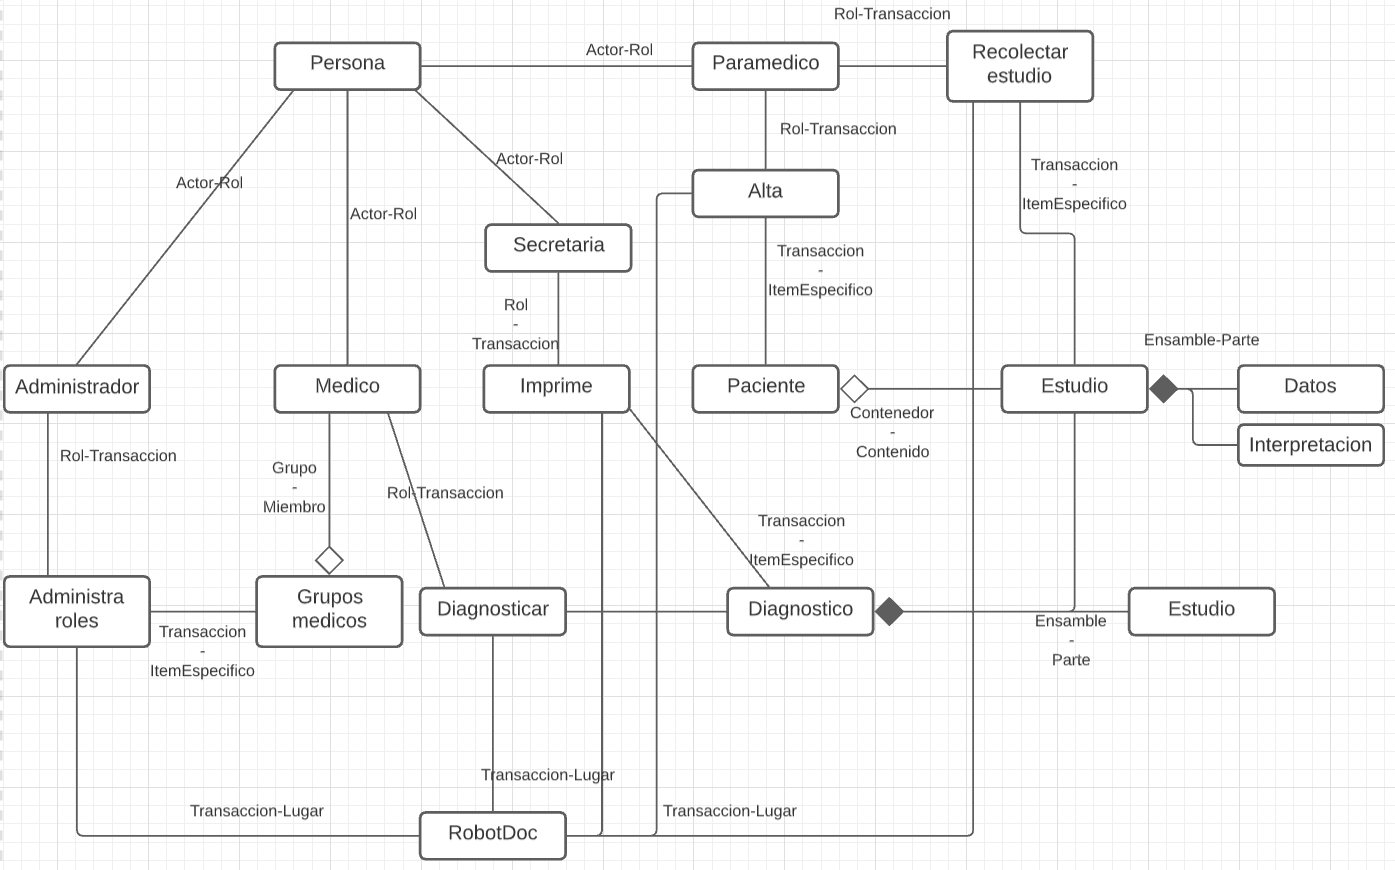
\includegraphics[width=\textwidth]{img/EjercicioRobotDoc.PNG}
\end{figure}


\begin{itemize}
\item Para ir armándolo siempre seguir los pasos.
\item El rol tiene que ver con la interacción con el sistema.
\item Se puede agregar también grupos de secretarias, y relacionar con secretaria
\end{itemize}

\subsection*{Arquitectura}


\begin{itemize}
\item Tenemos distintos niveles de abstracción, usaríamos el patrón Layer para resolver esta cuestión. Permitiendo desacoplar los recursos al encapsular en cada una de las capas (el layer).
\item Cada external server (Diagnosticos) tiene un MVC
\item Mas alto nivel es diagnostico
\item El microkernel esta compuesto por 3 componentes que deben de tener su sentido. Se debe de tener mas de una dirección de cambio. En nuestro caso se quiere conectar a aparatos nuevos, y nos dice que se van a hacer estudios nuevos. Por lo que es probable que tengamos que agregar médicos con especialidades nuevas.
\end{itemize}

\begin{figure}[!htb]
    \centering
    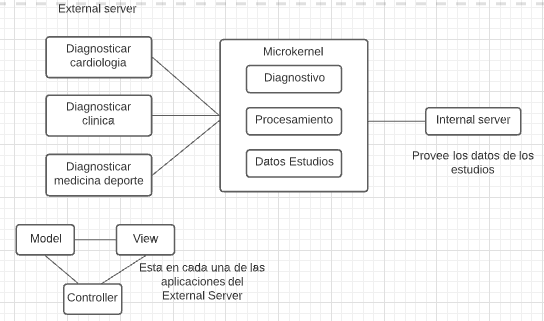
\includegraphics[width=0.8\textwidth]{img/EjercicioArquitectura.PNG}
\end{figure}

% hacer matriz
% no le pusimos reglas
% El hecho de que la arquitectura requiera flexibilidad va a tener impacto en las distintas vistas. (Esto ya lo implica la introducción del MVC)
% Hay un tema de seguridad tambien, y del manejo de señales

% (para ver como afectan las distintas vistas)